% Template for Cogsci submission with R Markdown

% Stuff changed from original Markdown PLOS Template
\documentclass[10pt, letterpaper]{article}

\usepackage{cogsci}
\usepackage{pslatex}
\usepackage{float}
\usepackage{caption}

% amsmath package, useful for mathematical formulas
\usepackage{amsmath}

% amssymb package, useful for mathematical symbols
\usepackage{amssymb}

% hyperref package, useful for hyperlinks
\usepackage{hyperref}

% graphicx package, useful for including eps and pdf graphics
% include graphics with the command \includegraphics
\usepackage{graphicx}

% Sweave(-like)
\usepackage{fancyvrb}
\DefineVerbatimEnvironment{Sinput}{Verbatim}{fontshape=sl}
\DefineVerbatimEnvironment{Soutput}{Verbatim}{}
\DefineVerbatimEnvironment{Scode}{Verbatim}{fontshape=sl}
\newenvironment{Schunk}{}{}
\DefineVerbatimEnvironment{Code}{Verbatim}{}
\DefineVerbatimEnvironment{CodeInput}{Verbatim}{fontshape=sl}
\DefineVerbatimEnvironment{CodeOutput}{Verbatim}{}
\newenvironment{CodeChunk}{}{}

% cite package, to clean up citations in the main text. Do not remove.
\usepackage{cite}

\usepackage{color}

% Use doublespacing - comment out for single spacing
%\usepackage{setspace}
%\doublespacing


% % Text layout
% \topmargin 0.0cm
% \oddsidemargin 0.5cm
% \evensidemargin 0.5cm
% \textwidth 16cm
% \textheight 21cm

\title{Adults and preschoolers seek visual information to support language
comprehension in noisy environments}


\author{ {\large \bf Kyle MacDonald}$^1$ (kylem4@stanford.edu), {\large \bf Virginia Marchman}$^1$ (marchman@stanford.edu),  \\ {\large \bf Anne Fernald}$^1$ (afernald@stanford.edu), {\large \bf Michael C. Frank}$^1$ (mcfrank@stanford.edu) 
  \\ $^1$ Department of Psychology Stanford University}

\begin{document}

\maketitle

\begin{abstract}
Language comprehension is a multisensory and interactive process. When
interpreting an utterance, listeners rapidly integrate information from
both the visual and the linguistic signals. But the quality of each
information source varies depending on the processing context, e.g.,
understanding speech in noise. Here, we present a strong test of the
hypothesis that listeners will adapt the dynamics of gaze during lexical
access to seek higher value visual information that supports
comprehension. We measured the timing and accuracy of adults (n=31) and
children's (n=40, 3-5 y.o.) eye movements during a real-time language
comprehension task and found that both age groups delayed the timing of
gaze shifts away from a speaker's face when processing speech in noise.
Interestingly, this delay resulted in higher information accumulation
from the visual signal, more accurate shifts, and fewer random eye
movements to the rest of the visual world. This results suggest that the
dynamics of gaze adapt to the processing demands of different contexts
and even young listeners will seek visual information that supports
real-time language comprehension.

\textbf{Keywords:}
eye movements; language processing; information-seeking; speech in
noise;
\end{abstract}

\section{Introduction}\label{introduction}

Real-time language comprehension is an interactive and multimodal
phenomenon. As skilled listeners, we continually integrate information
from both the visual and the linguistic signal in order to understand
what others are saying. A classic demonstration of this integration
process is the ``McGurk effect'' where a speaker's mouth movements
suggest one sound while their acoustic output suggests another. This
conflict results in the listener perceiving a third, intermediate sound
(J. MacDonald \& McGurk, 1978). Findings such as these have inspired
prominent theories of speech perception (McClelland, Mirman, \& Holt,
2006) and lexical processing (M. C. MacDonald \& Seidenberg, 2006;
Smith, Monaghan, \& Huettig, 2017) that argue for the fundamental role
of \emph{interactive} processes -- where listeners process information
from multiple sources in parallel. Moreover, empirical work on speech
perception shows that adults are better able to ``recover'' linguistic
information in noisy contexts when they have visual access to a
speaker's face (Erber, 1969)

However, the usefulness of integrating visual information varies
depending on features of the listener and features of the procssing
context. Consider the case of processing a visual-manual language like
American Sign Language (ASL). Here, the value of allocating visual
fixations to the language source (i.e., the signer) is incredibly high
since all of the language-relevant information is available in that
location. In our prior work, we showed that, compared to spoken language
learners, ASL-learners were more sensitive to the higher value of eye
movements in a visual language, choosing to prioritize information
accumulation and accuracy over and above speed when deciding to shift
gaze away from another signer (K. MacDonald, Blonder, Marchman, Fernald,
\& Frank, 2017). To explain this difference, we proposed an
information-seeking account inspired by goal-based theories of vision
(Hayhoe \& Ballard, 2005): that signers adapted the dynamics of gaze
during lexical access to seek information that supported accurate
language comprehension.

In the work reported here, we test a specific prediction of this
information-seeking account and ask whether listeners would adapt
patterns of fixation when looks to a speaker become more valuable -- as
is the case of processing speech in noise. Consider the familair example
of a speaker who asks you to ``Pass the salt'' in a noisy restaurant
where it is difficult to understand the request. The intuition is that
comprehension can be facilitated by gathering information via fixations
to the speaker by reading lips or perhaps the direction of gaze.

There has been recent interest in understanding how gaze patterns during
lexical access might adapt to different contexts that deviate from the
well-controlled lab settings that are typically used in psycholinguistic
tasks. For example, recent work by McMurray, Farris-Trimble, \& Rigler
(2017) shows that individuals with Cochlear Implants, who are
consistenly processing degraded auditory input, are more likely to delay
the process of lexical access as compared to listeners with typical
hearing. Our work asks a related question about whether the interaction
between language and visual attention interaction flexibly adapts to the
features of the processing context.

Specifically, we hypothesized that a noisy auditory environment would
make the auditory signal less reliable, and in turn increase the value
of fixating on a speaker for the task of language understanding. Our key
behavioral prediction is that listeners who process speech in noise will
delay generating an eye movement away from a speaker until they have
accumulated additional information about the named referent. In other
words, we predict that noisy contexts will lead to more fixations
allocated to a language-relevant aspect of the visual world. The next
section outlines the specific measurements and models that we use to
quantify the evidence for this hypothesis.

@ref(fig:stimuli\_plot)

\begin{CodeChunk}
\begin{figure*}[tb]

{\centering 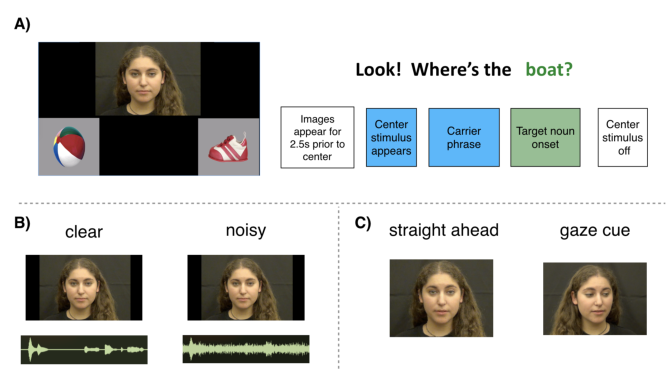
\includegraphics[width=0.8\linewidth]{figs/stimuli_plot-1} 

}

\caption[Stimuli for E1 and E2]{Stimuli for E1 and E2. Panel A shows the layout of the three fixation locations (speaker, target, and distracter), and the timecourse of a single trial. Panel B shows a visual representation of the clear and noisy waveforms used in E1. Panel C shows the gaze manipulation used in E2.}\label{fig:stimuli_plot}
\end{figure*}
\end{CodeChunk}

\section{Experiment}\label{experiment}

In this experiment we test whether our information-seeking account of
eye movements would generalize to a novel and ecologically valid
processing context -- speech in noise. We recorded eye movements during
a real-time language comprehension task where children and adults
processed familiar sentences (e.g., ``Where's the ball?'') while looking
at a simplified visual world with three fixation targets (see Fig 1).
Using a within-participants design, we manipulated the signal-to-noise
ratio of the auditory signal by convolving the language with brown
noise. We predicted that processing speech in noise would increase the
value of fixating on the speaker, causing listeners to gather additional
information before generating a shift to the named referent even after
the target word began unfolding in time.

To quantify evidence for our prediction, we compare the Accuracy and
Reaction Times (RTs) of participants' first shifts after target noun
onset between the noisy and clear contexts. We take a ``micro-level''
approach and use first shifts as window onto changes in the underlying
decision processes that generate eye movements. However, it is important
to point out that when we analyze differences in Accuracy, we are not
making claims about overall amount of time spent looking at the target
vs.~the distractor image -- a measure that is typically used in analyses
of the Visual World Paradigm.

We also present two model-based analyses that link the observable
behavior to underlying psychological constructs of interest. First, we
use an exponentially weighted moving average (EWMA) method
(Vandekerckhove \& Tuerlinckx, 2007) to classify participants' gaze
shifts as language-driven or random. In contrast to the standard
RT/Accuracy analysis, the EMWA approach allows us to quantify
participants' willingness to generate gaze shifts after noun onset but
before collecting sufficient information to seek the named referent.
Higher values indicate that participants were shifting early and equally
likely to land on the target or distractor image.

Next, we use drift-diffusion models (DDMs) (Ratcliff \& Childers, 2015)
to ask whether behavioral differences in Accuracy and RT are driven by a
more cautious responding strategy or by more efficient information
processing -- an important distinction for our theoretical account. We
predicted that processing speech in noise would make participants less
likely to shift before collecting sufficient information, leading to a
lower proportion of shifts flagged as random in the EWMA, and a higher
boundary separation estimate in the DDM, indicating a prioritization of
accuracy over and above speed.

\begin{CodeChunk}
\begin{figure*}[t]

{\centering 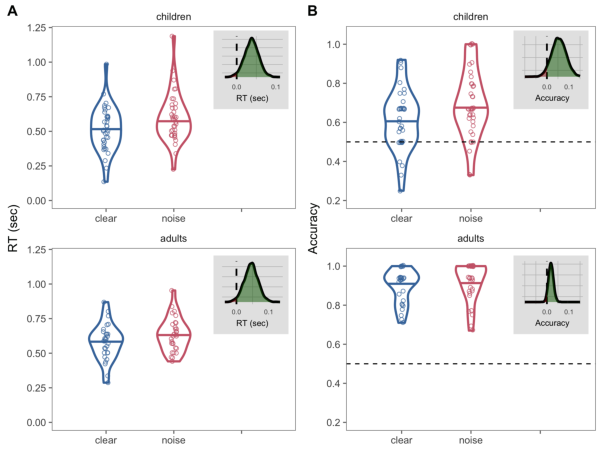
\includegraphics[width=0.85\linewidth]{figs/noise_acc_rt_e1_plot-1} 

}

\caption[Behavioral results for first shift Reaction Time (RT) and Accuracy]{Behavioral results for first shift Reaction Time (RT) and Accuracy. Panel A shows violin plots representing the distribution of RTs for each participant in each condition. Each black point represents a participant. The dark red points represent the model estimate for the group mean with the error bars showing the 95\% Highest Density Interval around that point estimate. The grey inset shows the full posterior distribution of the plausible RT differences across conditions with the vertical dashed line representing the null value of zero condition difference. The green shading represents estimates in the predicted direction and above the null value while the red shading represents estimates below the null. Panel B shows the same information but for Accuracy.}\label{fig:noise_acc_rt_e1_plot}
\end{figure*}
\end{CodeChunk}

\subsection{Method}\label{method}

\subsubsection{Participants}\label{participants}

Participants were native, monolingual English-learning children (\(n=\)
39; 22 F, 17 M) and adults (\(n=\) 31; 22 F, 9 M). All participants had
no reported history of developmental or language delay and normal
vision. 14 participants (11 children, 3 adults) were run but not
included in the analysis because either the eye tracker falied to
calibrate or the participant did not complete the task.

\subsubsection{Stimuli}\label{stimuli}

\emph{Linguistic stimuli.} The video/audio stimuli were recorded in a
sound-proof room and featured two female speakers who used natural
child-directed speech and said one of two phrases: ``Hey! Can you find
the (target word)'' or ``Look! Where's the (target word) -- see panel A
of Fig 1. The target words were: ball, bunny, boat, bottle, cookie,
juice, chicken, and shoe. The target words varied in length (shortest =
411.68 ms, longest = 779.62 ms) with an average length of 586.71 ms.

\emph{Noise manipulation}. To create the stimuli in the noise condition,
we convolved each recording with Brown noise using the Audacity audio
editor. The average signal-to-noise ratio\footnote{The ratio of signal
  power to the noise power, with values greater than 0 dB indicating
  more signal than noise.} in the noise condition was 2.87 dB compared
to the clear condition, which was 35.05 dB.

\emph{Visual stimuli.} The image set consisted of colorful digitized
pictures of objects presented in fixed pairs with no phonological
overlap between the target and the distractor image (cookie-bottle,
boat-juice, bunny-chicken, shoe-ball). The side of the target picture
was counterbalanced across trials.

\subsubsection{Design and procedure}\label{design-and-procedure}

Participants viewed the task on a screen while their gaze was tracked
using an SMI RED corneal-reflection eye-tracker mounted on an LCD
monitor, sampling at 60 Hz. The eye-tracker was first calibrated for
each participant using a 6-point calibration. On each trial,
participants saw two images of familiar objects on the screen for two
seconds before the center stimulus appeared (see Fig 1). Next, they
processed the target sentence -- which consisted of a carrier phrase, a
target noun, and a question -- followed by two seconds without language
to allow for a response. Child participants saw 32 trials (16 noise
trials; 16 clear trials) with several filler trials interspersed to
maintain interest. Adult participants saw 64 trials (32 noise; 32
clear). The noise manipulation was presented in a blocked design with
the order of block counterbalanced across participants.

\subsection{Results and Discussion}\label{results-and-discussion}

\subsubsection{Analysis plan}\label{analysis-plan}

First, we present behavioral analyses of First Shift Accuracy and
Reaction Time (RT).\footnote{See \url{https://osf.io/g8h9r/} for a
  pre-registration of the analysis plan.} RT corresponds to the latency
to shift away from the central stimulus to either picture measured from
the onset of the target noun. (all RTs were analyzed in log space).
Accuracy corresponds to whether participantss first gaze shifta landed
on the target or the distracter picture. We used the \texttt{rstanarm}
(Gabry \& Goodrich, 2016) package to fit Bayesian mixed-effects
regression models. The mixed-effects approach allowed us to model the
nested structure of our data -- multiple trials for each participant and
item, and a within-participants manipulation -- by including random
intercepts for each participant and item, and a random slope for each
item and noise condition. We used Bayesian estimation to quantify
uncertainty in our point estimates, which we communicate using a 95\%
Highest Density Interval (HDI). The HDI provides a range of credible
values given the data and model. All analysis code can be found in the
online repository for this project:
\url{https://github.com/kemacdonald/speed-acc/R/analysis}.

Next, we present the two model-based analyses -- the EWMA and DDM. The
goal of these models is to move beyond a description of the data and map
behavioral differences in eye movements to underlying psychological
variables. The EWMA method models changes in random shifting behavior as
a function of RT. For each participant, the model classifies the
proportion of shifts that were likely to be language-driven as opposed
to random responding, which we call the \emph{guessing} parameter.

\begin{CodeChunk}
\begin{figure}[t]

{\centering 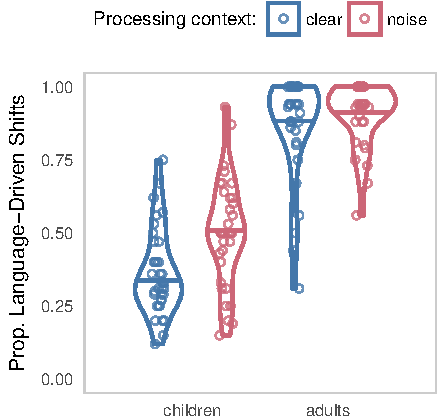
\includegraphics[width=0.85\linewidth]{figs/ewma_violin_plot-1} 

}

\caption[EWMA results for children and adults]{EWMA results for children and adults. Each point represents the proportion of shifts categorized as guessing for a single participant. The color of the violin plot represents the processing context: noise vs. clear.}\label{fig:ewma_violin_plot}
\end{figure}
\end{CodeChunk}

\begin{CodeChunk}
\begin{figure}[t]

{\centering 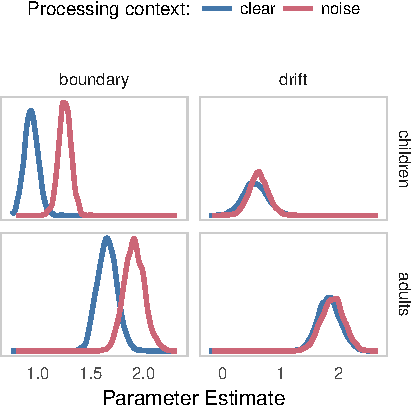
\includegraphics[width=0.85\linewidth]{figs/hddm_plot_noise-1} 

}

\caption[HDDM results]{HDDM results. Each panel shows the posterior distribution for either the boundary separation or drift rate parameters for children (top panels) and adults (bottom panels).}\label{fig:hddm_plot_noise}
\end{figure}
\end{CodeChunk}

After fitting the EWMA, we took the shifts that were categorized as
language-driven and fit a hierarchical Bayesian drift-diffusion model
(HDDM). This model quantifies differences in separable parameters of the
underlying decision process that lead to different patterns of behavior.
The model assumes that people accumulate noisy evidence in favor of one
alternative with a response generated when the evidence crosses a
pre-defined decision threshold. Here, we focus on two parameters of
interest: \textbf{boundary separation}, which indexes the amount of
evidence gathered before generating a response (higher values suggest
more cautious responding) and \textbf{drift rate}, which indexes the
amount of evidence accumulated per unit time (higher values suggest more
efficient processing).

\subsubsection{Behavioral analyses}\label{behavioral-analyses}

\textbf{RT.} To make RTs more suitable for modeling on a linear scale,
we analyzed responses in log space with the final model specified as:
\texttt{$log(RT) \sim noise\_condition + age\_group + (sub\_id + noise\_condition \mid item)$}.
Panel A of Figure 2 shows the full RT data distribution, the estimates
of condition means, and the full posterior distribution of the estimated
difference between the noise and clear conditions. Both children and
adults were slower to identify the target in the noise condition
(Children \(M_{noise}\) = 0.5 ms; Adult \(M_{noise}\) = 0.6 ms), as
compared to the clear condition (Children \(M_{clear}\) = 0.46 ms; Adult
\(M_{clear}\) = 0.55 ms). RTs in the noise condition were 41.73 ms
slower on average, with a 95\% HDI from 1.19 ms to 82.26 ms that did not
include the null value of zero condition difference.

\textbf{Accuracy.} Next, we modeled adults' and children's first shift
accuracy using a mixed-effects logistic regression with the same
specifications (see Panel B of Fig 2). Both groups were more accurate
than a model of random responding (null value of \(0.5\) falling well
outside the lower bound of the 95\% HDI for all group means). Adults
were more accurate (\(M_{adults} =\) 90\%) than children
(\(M_{children} =\) 62\%). The key result is that both groups showed
evidence of higher accuracy in the noise condition (Children
\(M_{noise}\) = 67\%; Adult \(M_{noise}\) = 92\%) as compared to the
clear condition (Children \(M_{clear}\) = 62\%; Adult \(M_{clear}\) =
90\%). Accuracy in the noise condition was 4\% higher on average, with a
95\% HDI from 0\% to 11\%. Note that the null value of zero difference
falls at the very edge of the 95\% HDI such that 95\% of the credible
values fall below the null, providing evidence for higher accuracy in
the noise condition.

\subsubsection{Model-based analyses}\label{model-based-analyses}

\textbf{EWMA.} Figure 3 shows the proportion of shifts that the model
classified as random vs.~language-driven for each age group and
processing contxt. Critically, processing speech in noise caused both
adults and children to produce a higher proportion of language-driven
shifts with the 95\% HDI excluding the null value (see Table 1). This
pattern suggests that the noise condition led participants to increase
visual fixations to the language source, leading them to generate fewer
exploratory, random shifts before accumulating sufficient information to
respond accurately.

\textbf{HDDM.} Figure 4 shows the full posterior distributions for the
HDDM output. Children had lower drift rates and boundary separation
estimates as compared to adults, suggesting that children were less
efficient and less cautious in their responding (see also Table 2).
Intrestingly, the noise manipulation only affected the boundary
separation parameter, with higher estimates in the noise condition for
both age groups. This result suggests that participants' in the noise
condition prioritized information accumulation over speed when
generating an eye movement in response to the incoming language. This
increased decision threshold led to higher accuracy. Moreover, the high
overlap in estimates of drift rate suggests that participants were able
to integrate the visual and auditory signals such that they could
achieve a level of processing efficiency comparable to the clear
processing context.

Together, the behavioral and EWMA/HDDM results provide converging
support for the predictions of our information-seeking account. In
summary, processing speech in noise caused listeners to seek additional
visual information to support language comprehension. Moreover, we
observed a strikingly similar pattern of behavior in children and
adults, with both groups producing more language-driven shifts and
prioritizing accuracy over speed in the more challenging, noisy context.
These data have interesting parallels to recent work from McMurray et
al. (2017), showing that adults with Cochlear Implants, who consistently
process degraded auditory input, will delay lexical access and wait
until substantial information has accumulated. This process is in
contrast to the ``immediate competition'' model of word recognition
where listeners activate candidate meanings from word onset.

\begin{table}[t]
\centering
\begin{tabular}{llr}
  \hline
Parameter & Contrast & Estimate (95\% HDI) \\ 
  \hline
Cut point & age group & 0.21 [0.18, 0.24] \\ 
  Cut point & noise & 0.04 [0.01, 0.06] \\ 
  Guessing & adults-children & 0.46 [0.43, 0.49] \\ 
  Guessing & noise-clear & 0.12 [0.07, 0.17] \\ 
   \hline
\end{tabular}
\caption{EWMA results for E1 and E2. The guessing parameter refers to the proportion of gaze shifts classified as random vs. language-driven with higher values indicating more random responding. Estimate refers to the difference between condition or age group.} 
\end{table}

\section{General Discussion}\label{general-discussion}

Language comprehension in grounded contexts involves integrating the
visual and linguistic signals. But the value of gathering visual
information can vary depending on features of the processing context.
Here, we presnted a strong test of an information-seeking account of eye
movements during language processing -- an ccount that we first proposed
in K. MacDonald et al. (2017) to explain population-level differences in
the dynamics of gaze between children learning ASL and children learning
spoken English. Here, we showed that children and adults adapt to
processing speech in noise by producing slower but more accurate gaze
shifts away from a speaker. Both groups also showed evidence of
prioritizing information accumulation over speed (HDDM) while producing
more language driven shifts (EWMA). It is interesting that listeners
were able to achieve higher accuracy in the more challenging, noisy
context. Together, the behavioral and modeling results suggest that when
the linguistic signal is degraded, listeners adapt their eye movements
to seek language-relevant information in the visual world.

\begin{table}[t]
\centering
\begin{tabular}{lllr}
  \hline
Parameter & Condition & Age Group & Estimate [95\% HDI] \\ 
  \hline
boundary & clear & adults & 1.68 [1.5, 1.87] \\ 
  boundary & clear & children & 0.96 [0.84, 1.09] \\ 
  boundary & noise & adults & 1.65 [1.48, 1.83] \\ 
  boundary & noise & children & 1.23 [1.12, 1.34] \\ 
   \hline
drift & clear & adults & 1.86 [1.48, 2.25] \\ 
  drift & clear & children & 0.58 [0.17, 0.99] \\ 
  drift & noise & adults & 1.94 [1.56, 2.33] \\ 
  drift & noise & children & 0.59 [0.27, 0.93] \\ 
   \hline
\end{tabular}
\caption{HDDM parameter estimates for each age group and noise condition. The drift rate parameter indexes processing efficiency and the boundary separation parameter indexes participants' information accumulation threshold.} 
\end{table}

These results bring together ideas from several research programs.
First, work on language-mediated visual attention shows that adults and
children rapidly shift gaze upon hearing the name of an object in the
visual scene (Allopenna, Magnuson, \& Tanenhaus, 1998; Tanenhaus,
Spivey-Knowlton, Eberhard, \& Sedivy, 1995). The speed and consistency
of this response has led to debates about whether language-mediated gaze
shifts are automatic as opposed to under the control of the listener.
While we do claim that listeners in our task have explicit access to the
underlying decision process, our findings show that the dynamics of gaze
during lexical access adapt to the information features of the context.
This finding parallels recent work by McMurray et al. (2017), showing
that adults with Cochlear Implants, who consistently process degraded
auditory input, will delay the process of lexical access, waiting to
begin until substantial information has accumulated.

Second, empirical work on vision during natural tasks shows that people
overwhelmingly prefer to look at \emph{goal-relevant} locations -- e.g.,
an upcoming obstacle while walking (Hayhoe \& Ballard, 2005). These
accounts inspired our prediction that gaze dynamics during language
comprehension should adapt to the value of different fixation behaviors
with respect to the listener's goal of rapid language processing. And
third, work on effortful listening shows that listeners generate
compensatory responses (e.g., increases in attention and working memory)
within ``challenging'' comprehension contexts such as processing noisy
or accented speech (Van Engen \& Peelle, 2014). These accounts predict
that our young listeners might compensate for the reduced quality of the
auditory signal by allocating gathering additional visual information.

This work has several important limitations that we hope will pave the
way for future work. Here, we chose to focus on a single decision about
visual fixation to provide a window onto the underlying dynamics of
decision-making across different processing contexts. However, the
decision to shift away from a language is just one of the many decisions
that listeners make while processing language in real-time. Moreover,
our micro-level analysis does not consider the rich gaze patterns that
occur before this decision. In our future work, we aim to quantify
changes in the dynamics of gaze across the full sentence processing
context. Finally, we used a simple visual world, with only three places
to look, and very simple linguistic stimuli, especially for the adults.
Thus it remains an open question how these results might scale up to
more complex language information and visual environments.

We designed this experiment as a strong test our
information-maximization proposal in the domain of familiar language
comprehension. However, we think that the account is more general. And
we are interested in applying this framework -- the in-depth analysis of
decisions about visual fixation -- to the language acquisition context.
Consider that early in language learning children are acquiring novel
word-object links while also learning about visual object categories.
Both of these tasks produce goals that should in turn modulate
children's decisions about where to allocate visual attention, e.g.,
seeking nonlinguistic cues to reference such as eye gaze and pointing
become critical when you are unfamiliar with the information in the
linguistic signal. More generally, we think that these results
contribute to a recent theoretical emphasis on including goal-based
accounts of eye movements during language comprehension (Salverda,
Brown, \& Tanenhaus, 2011). We hope that our approach presents a way
forward for explaining fixation behaviors across a wider variety of
populations, processing contexts, and during different stages of
language learning.

\section{Acknowledgements}\label{acknowledgements}

We are grateful to the families who participated in this research.
Thanks to Tami Alade and Hannah Slater for help with data collection.
This work was supported by an NSF GRFP to KM.

\section{References}\label{references}

\setlength{\parindent}{-0.1in} \setlength{\leftskip}{0.125in} \noindent

\hypertarget{refs}{}
\hypertarget{ref-allopenna1998tracking}{}
Allopenna, P. D., Magnuson, J. S., \& Tanenhaus, M. K. (1998). Tracking
the time course of spoken word recognition using eye movements: Evidence
for continuous mapping models. \emph{Journal of Memory and Language},
\emph{38}(4), 419--439.

\hypertarget{ref-erber1969interaction}{}
Erber, N. P. (1969). Interaction of audition and vision in the
recognition of oral speech stimuli. \emph{Journal of Speech and Hearing
Research}, \emph{12}(2), 423--425.

\hypertarget{ref-gabry2016rstanarm}{}
Gabry, J., \& Goodrich, B. (2016). Rstanarm: Bayesian applied regression
modeling via stan. r package version 2.10. 0.

\hypertarget{ref-hayhoe2005eye}{}
Hayhoe, M., \& Ballard, D. (2005). Eye movements in natural behavior.
\emph{Trends in Cognitive Sciences}, \emph{9}(4), 188--194.

\hypertarget{ref-macdonald1978visual}{}
MacDonald, J., \& McGurk, H. (1978). Visual influences on speech
perception processes. \emph{Attention, Perception, \& Psychophysics},
\emph{24}(3), 253--257.

\hypertarget{ref-macdonald2017info}{}
MacDonald, K., Blonder, A., Marchman, V. and, Fernald, A., \& Frank, M.
C. (2017). An information-seeking account of eye movements during spoken
and signed language comprehension. In \emph{Proceedings of the 39th
annual conference of the cognitive science society}.

\hypertarget{ref-macdonald2006constraint}{}
MacDonald, M. C., \& Seidenberg, M. S. (2006). Constraint satisfaction
accounts of lexical and sentence comprehension. \emph{Handbook of
Psycholinguistics}, \emph{2}, 581--611.

\hypertarget{ref-mcclelland2006there}{}
McClelland, J. L., Mirman, D., \& Holt, L. L. (2006). Are there
interactive processes in speech perception? \emph{Trends in Cognitive
Sciences}, \emph{10}(8), 363--369.

\hypertarget{ref-mcmurray2017waiting}{}
McMurray, B., Farris-Trimble, A., \& Rigler, H. (2017). Waiting for
lexical access: Cochlear implants or severely degraded input lead
listeners to process speech less incrementally. \emph{Cognition},
\emph{169}, 147--164.

\hypertarget{ref-ratcliff2015individual}{}
Ratcliff, R., \& Childers, R. (2015). Individual differences and fitting
methods for the two-choice diffusion model of decision making.
\emph{Decision}, \emph{2}(4), 237--279.

\hypertarget{ref-salverda2011goal}{}
Salverda, A. P., Brown, M., \& Tanenhaus, M. K. (2011). A goal-based
perspective on eye movements in visual world studies. \emph{Acta
Psychologica}, \emph{137}(2), 172--180.

\hypertarget{ref-smith2017multimodal}{}
Smith, A. C., Monaghan, P., \& Huettig, F. (2017). The multimodal nature
of spoken word processing in the visual world: Testing the predictions
of alternative models of multimodal integration. \emph{Journal of Memory
and Language}, \emph{93}, 276--303.

\hypertarget{ref-tanenhaus1995integration}{}
Tanenhaus, M. K., Spivey-Knowlton, M. J., Eberhard, K. M., \& Sedivy, J.
C. (1995). Integration of visual and linguistic information in spoken
language comprehension. \emph{Science}, \emph{268}(5217), 1632.

\hypertarget{ref-van2014listening}{}
Van Engen, K. J., \& Peelle, J. E. (2014). Listening effort and accented
speech. \emph{Frontiers in Human Neuroscience}, \emph{8}.

\hypertarget{ref-vandekerckhove2007fitting}{}
Vandekerckhove, J., \& Tuerlinckx, F. (2007). Fitting the ratcliff
diffusion model to experimental data. \emph{Psychonomic Bulletin \&
Review}, \emph{14}(6), 1011--1026.

\end{document}
